
% --------------------------------------------------------------------
% This is a simple Beamer document that uses beamerthemesigma.sty
% Reading the comments should help you create a presentation even if
% you've never used Beamer before.
% --------------------------------------------------------------------
% Set our document class to Beamer
\documentclass[aspectratio=169]{beamer}

% Some packages for nice font encodings in the final PDF
\usepackage[utf8]{inputenc}
\usepackage[T1]{fontenc}

% From Jeff E
\usepackage{algo}

\usepackage{sigmastyle}

% To insert images
\usepackage{graphicx}

% Useful packages from the AMS
\usepackage{amsmath,amssymb,amsthm}

% Package for code highlighting
\usepackage{minted}
\setminted{linenos=true, breaklines=true, breakanywhere=true, style=default}
\usemintedstyle{monokai}

% Set a title
\title{Decidability and Reductions}

% The subtitle is generally where I'd expect you to put the week
% number, thus:
\subtitle{Week 8}
% \texorpdfstring to remove compilation warnings if you have math here

% Whoever worked on the presentation:
\author{Anakin}

% A date, if you'd like.
\date{}

% An institute name, if you're so inclined
% \institute{University of Illinois Urbana-Champaign}

% Use the SIGma theme for this Beamer presentation
\usetheme{sigma}
% --------------------------------------------------------------------
% Begin document
\begin{document}

% Beamer calls each slide a "frame", defined within the environment:
% \begin{frame}
%   <frame content here>
% \end{frame}

% This frame is just the title.
\begin{frame}
\titlepage
\end{frame}

% A frame with the table of contents.
% This frame's title is "Outline".
\begin{frame}{Outline}
  \tableofcontents
\end{frame}

\section{Decidability \& Recognizability}
\frame{\sectionpage}

% Not sure if I want these slides
% \begin{frame}{Quick Review}
%     What are Turing Machines?
%     \begin{itemize}
%         \item The fundamental basis for all models of computation. \pause
%         \item Extremely barebones design
%         \begin{itemize}
%             \item As such, writing programs gets tedious very quickly \pause
%         \end{itemize}
%         \item For all intents and purposes, essentially computer programs
%         \begin{itemize}
%             \item So we'll speak about them like normal computers \pause
%         \end{itemize}
%         \item They allow us to reason about what we can and cannot compute
%     \end{itemize}
% \end{frame}

\begin{frame}
  \frametitle{Turing Machine}
  \begin{center}
    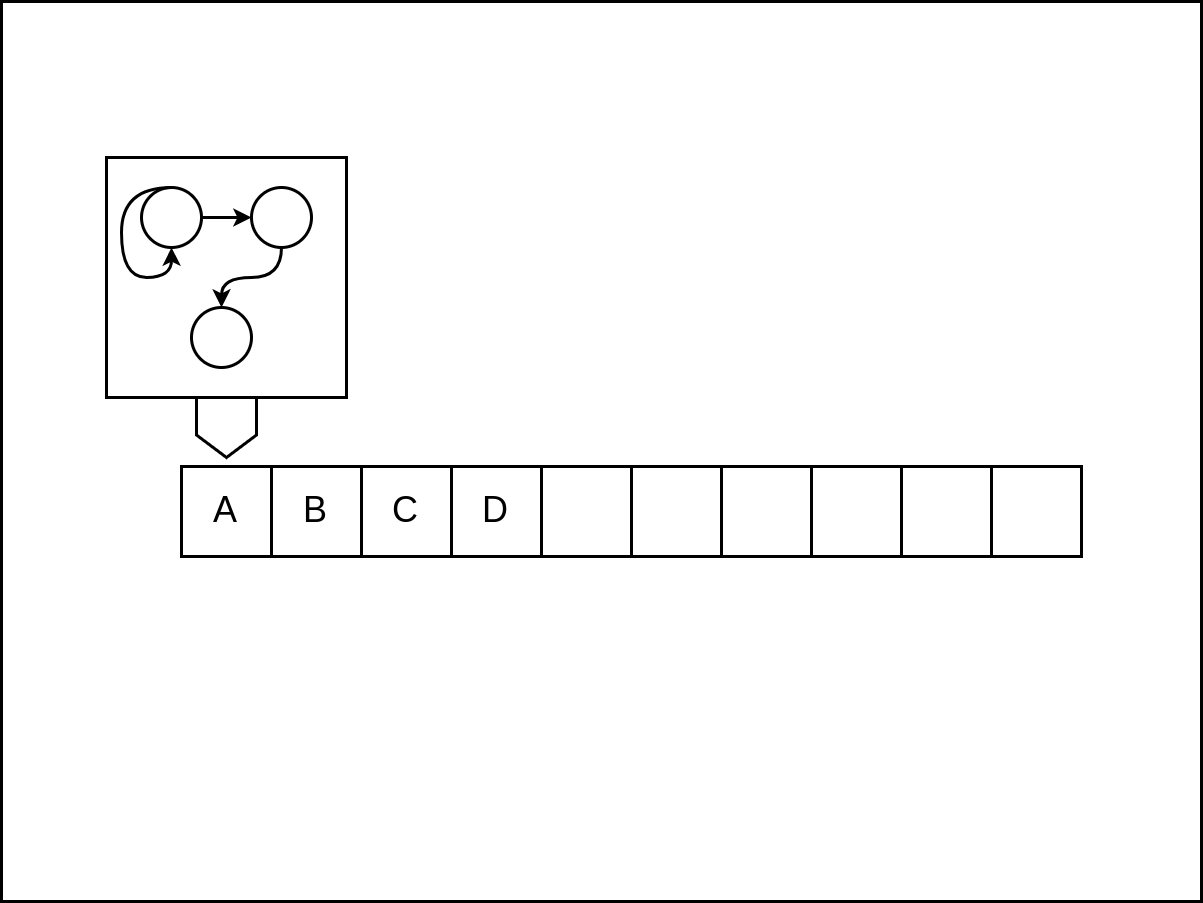
\includegraphics[width=.75\textwidth]{frame1.png}
  \end{center}
\end{frame}

\begin{frame}
  \frametitle{Turing Machine}
  \begin{center}
    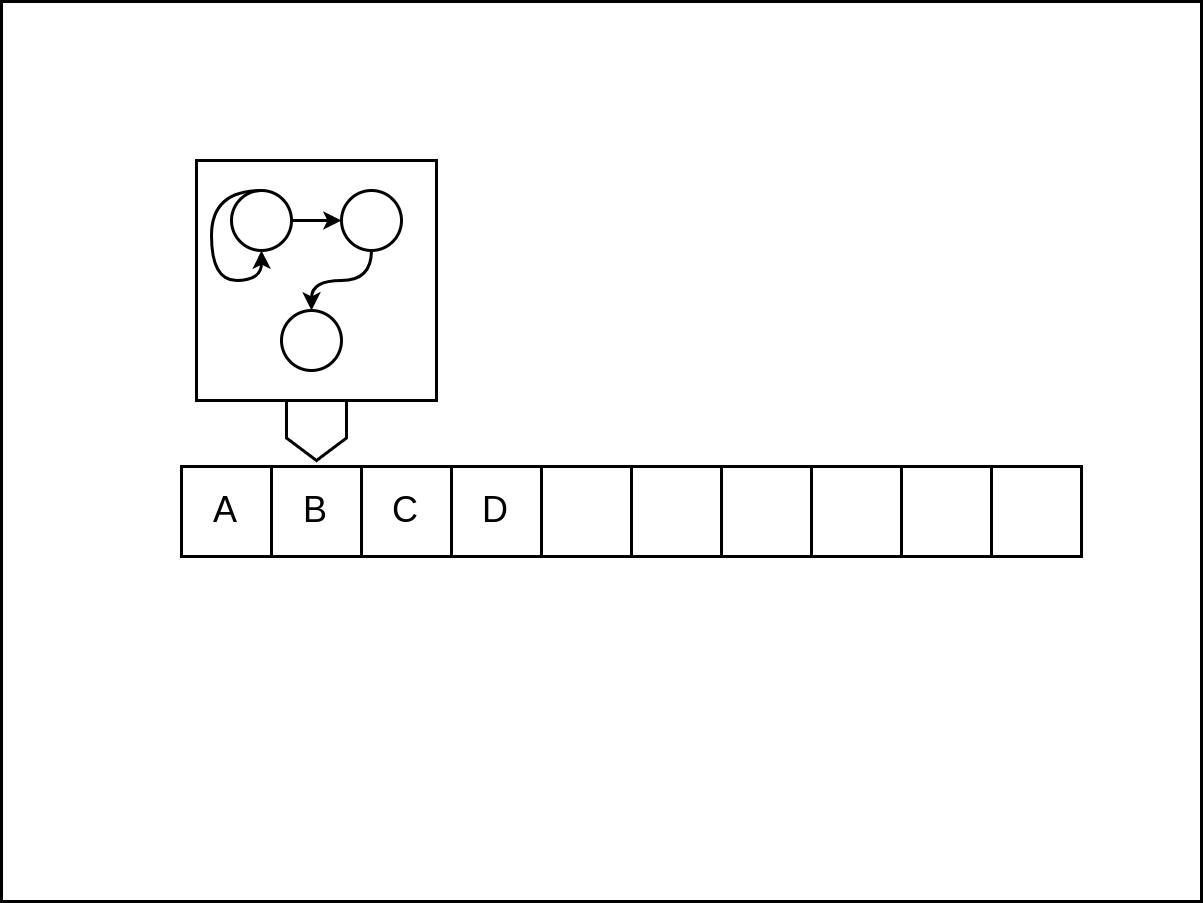
\includegraphics[width=.75\textwidth]{frame2.png}
  \end{center}
\end{frame}

\begin{frame}
  \frametitle{Turing Machine}
  \begin{center}
    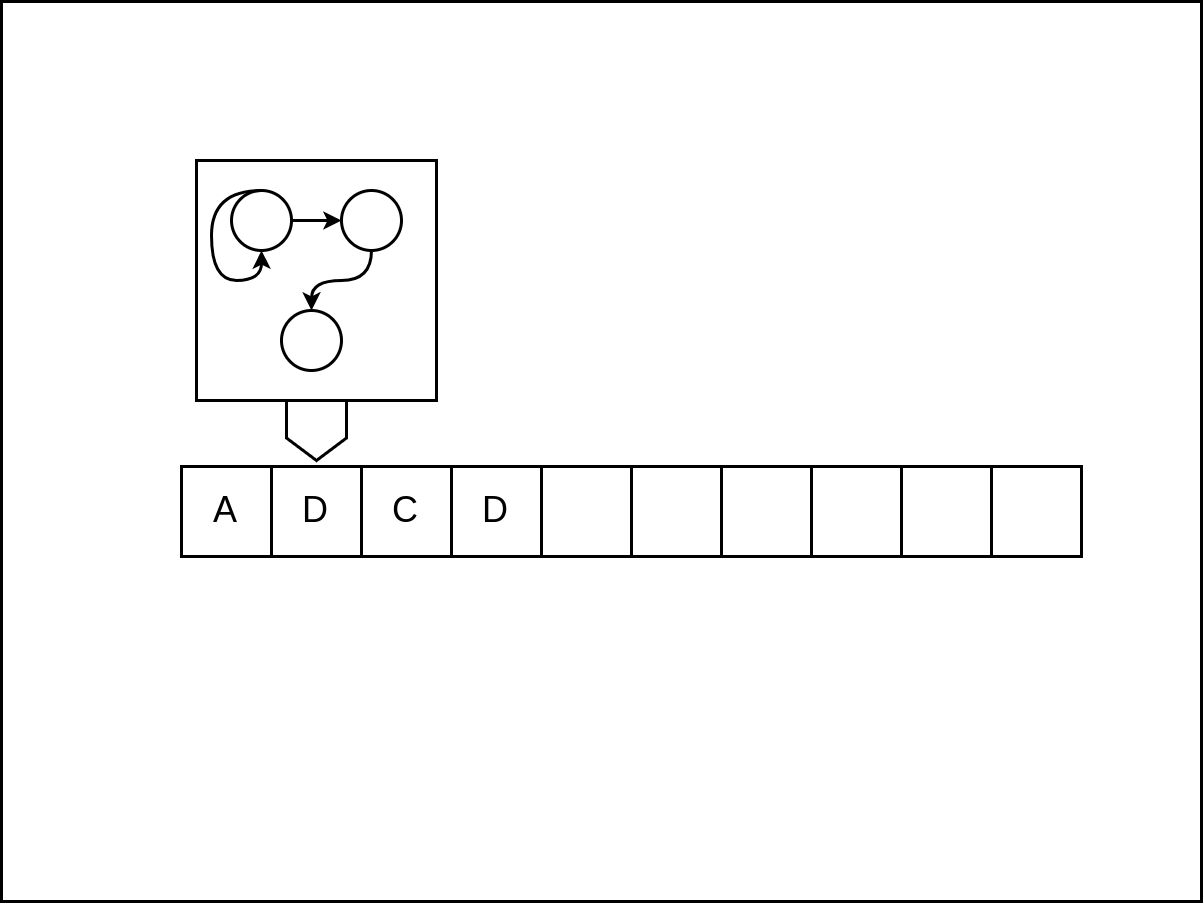
\includegraphics[width=.75\textwidth]{frame3.png}
  \end{center}
\end{frame}

\begin{frame}
  \frametitle{Turing Machine}
  \begin{center}
    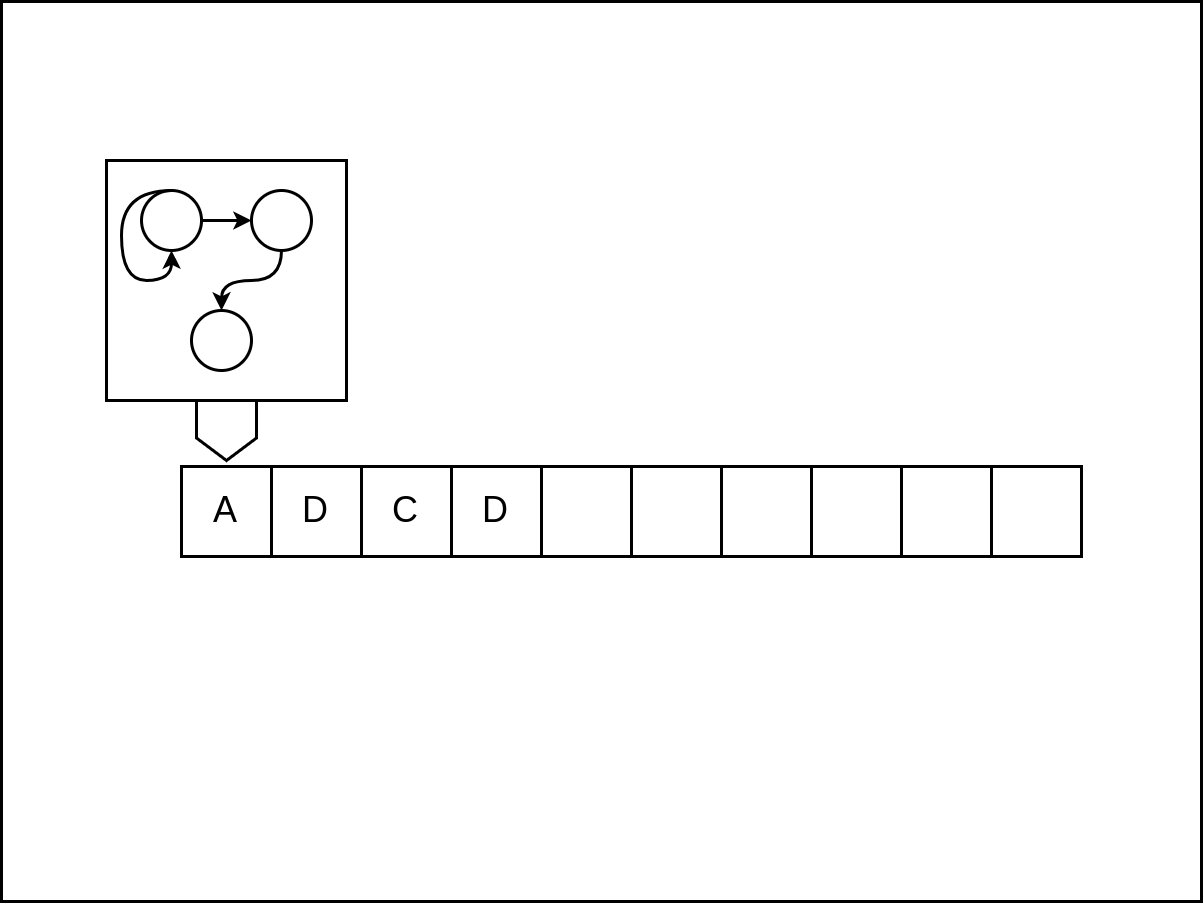
\includegraphics[width=.75\textwidth]{frame4.png}
  \end{center}
\end{frame}

\begin{frame}
  \frametitle{Turing Machine}
  \begin{center}
    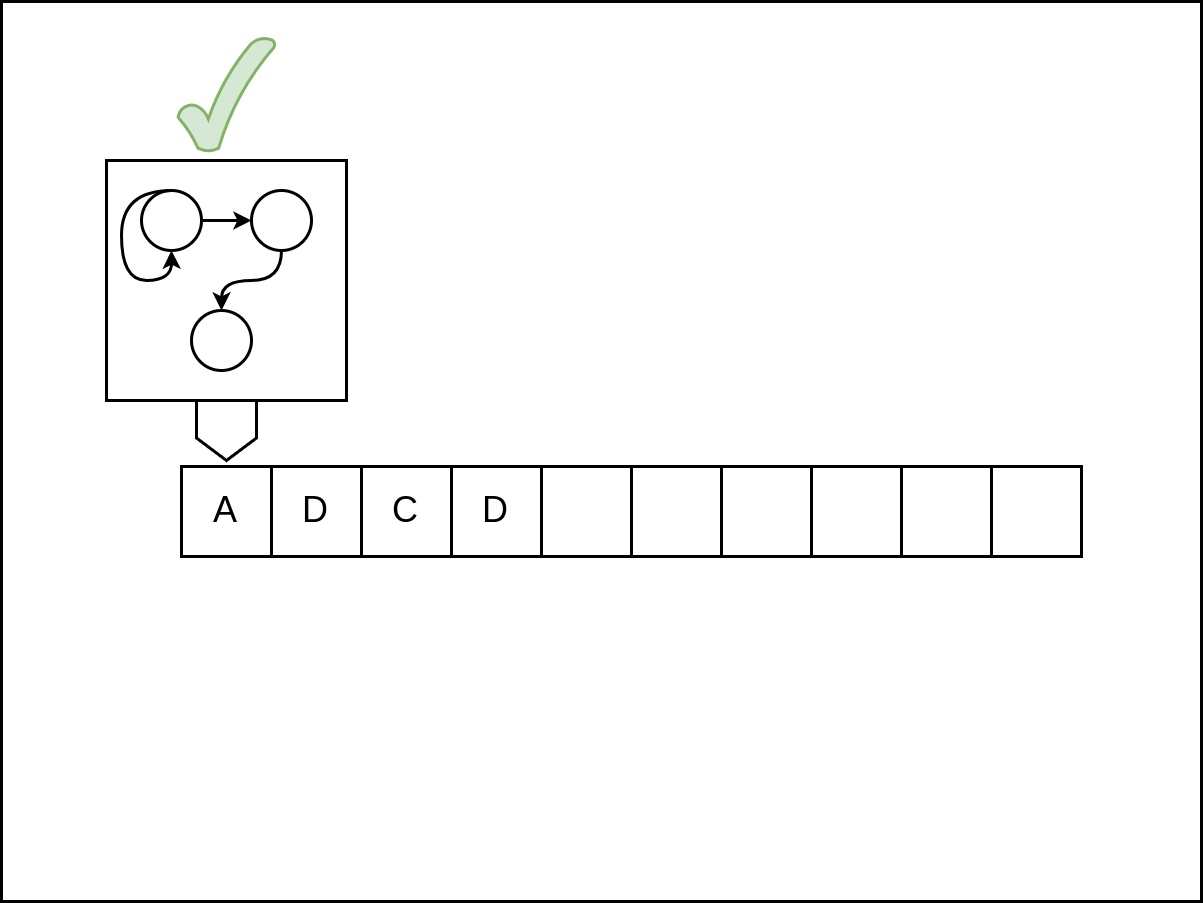
\includegraphics[width=.75\textwidth]{frame5.png}
  \end{center}
\end{frame}

\begin{frame}{Languages}
    \begin{itemize}
        \item Like all the other machines we've seen before, we can talk about their \textbf{languages}
        \item However, there is some more subtlety \pause
        \begin{itemize}
            \item \textsc{Accept($M$)}: the language of all inputs $w$ where $M$ accepts. \pause
            \item \textsc{Reject($M$)}: the language of all inputs $w$ where $M$ rejects. \pause
            \item \textsc{Halt($M$)}: the language of all inputs $w$ where $M$ halts.
            \begin{itemize}
                \item \textsc{Halt($M$)} $=$ \textsc{Accept($M$)} $\cup$ \textsc{Reject($M$)} \pause
            \end{itemize}
            \item \textsc{Diverge($M$)}: the language of all inputs $w$ where $M$ never halts.
    \end{itemize}
    \end{itemize}
\end{frame}

\begin{frame}{Decision Languages}
    If a problem only has a true or false response, we can talk about the \textbf{decision language} of that problem: \pause
    
    \begin{align*}
        \textsc{SAT} &= \{w \in \Sigma^* \mid w \text{ is a satisfiable boolean formula}\} \\
        \textsc{SORT} &= \{w \in \Sigma^* \mid w \text{ defines a sorted integer array}\} \\
        \textsc{HALT} &=  \{w \in \Sigma^* \mid w \text{ is a program that halts}\}
    \end{align*}
\end{frame}

\begin{frame}{Recognizability and Decidability}
    \begin{itemize}
        \item We say that $M$ \textbf{\textit{recognizes/accepts}} $L$ if for any input $w\in L$, $M$ accepts $w$. \pause
        \begin{itemize}
            \item If $w \in L$, then $M$ must \textbf{accept} $w$
            \item If $w \notin L$, then $M$ can \textbf{reject} or even \textbf{never halt} \pause
        \end{itemize}
        \item $M$ \textbf{\textit{decides}} $L$ if for any input $w$, $M$ accepts if $w \in L$ and rejects otherwise.
        \begin{itemize}
            \item If $w \in L$, then $M$ must \textbf{accept} $w$
            \item If $w \notin L$, then $M$ must \textbf{reject} $w$ \pause
            \item Either way, $M$ must halt on all inputs
        \end{itemize}
    \end{itemize}
\end{frame}

\begin{frame}{Classifying Languages}
    \begin{itemize}
        \item $L$ is \textbf{recognizable} if there exists some TM $M$ that recognizes it \pause
        \item $L$ is \textbf{decidable} if there exists some TM $M$ that decides it
    \end{itemize}
\end{frame}

\begin{frame}{Examples}
    \begin{itemize}
        \item $\set{n | n \in \mathbb{Z} \text{ and $n$ is even}}$ 
        \begin{itemize}
            \item This is decidable
        \end{itemize} \pause
        \item $A_{\text{TM}} = \set{\langle M, w \rangle | \text{$M$ is a TM and $M$ accepts $w$}}$
        \begin{itemize}
            \item This is recognizable \pause
            \item It is NOT decidable (we'll see why later)
        \end{itemize}
    \end{itemize}
\end{frame}

\begin{frame}{}
    \begin{center}
        {\color{sigma@mainblue} \LARGE Questions?}
    \end{center}
\end{frame}

\section{The Halting Problem}
\frame{\sectionpage}

\begin{frame}{What is The Halting Problem?}
    \begin{itemize}
        \item In 1928 at the Second International Congress of Mathematicians in Paris, David Hilbert posed the ``Entscheidungsproblem'' asking ``is mathematics decidable?'' \pause
        \item Alan Turing in 1936 showed that a solution to the Entscheidungsproblem is \textbf{impossible} 
        \begin{itemize}
            \item Alonzo Church independently proved this 3 months prior
        \end{itemize} \pause
        \item We are going to look the proof of this today 
    \end{itemize}
\end{frame}

\begin{frame}{The Language \emph{HALT}}
    \begin{itemize}
        \item Showing that a language is decidable is easy
        \begin{itemize}
            \item Just build a decider
        \end{itemize} \pause
        \item Showing that a language is undecidable is much harder
        \begin{itemize}
            \item You have to show no machine can decide the language, no matter what you try (done using contradiction).
        \end{itemize} \pause
        \item $HALT = \set{\langle M, w \rangle | \text{$M$ is a TM and $M$ halts on input $w$}}$
        \begin{itemize}
        \item We will show this language is undecidable
        \end{itemize} 
    \end{itemize}
\end{frame}

\begin{frame}{The Proof}
    Suppose \emph{HALT} is decidable. Then we have a Turing Machine $\textsc{H}$ that decides it:
    \begin{algo}
        \underline{\textsc{H}$(\langle M, w \rangle)$}:\+
    \\      If $M$ halts on input $w$:\+
    \\          return \emph{accept}\-
    \\      else:\+
    \\          return \emph{reject}
    \end{algo}
\end{frame}

\begin{frame}{The Proof}
    Using $\textsc{H}$, we can build a new machine $\textsc{SelfHalt}$:
    \begin{algo}
        \underline{\textsc{SelfHalt}$(\langle M \rangle)$}:\+
    \\      return \textsc{H}$(\langle M, M \rangle)$
    \end{algo} \pause
    
    Then we can build a machine \textsc{OPP} that does the opposite of \textsc{SelfHalt}
    \begin{algo}
        \underline{\textsc{Opp}$(\langle M \rangle)$}:\+
    \\      If \textsc{SelfHalt}$(\langle M \rangle)$ accepts:\+
    \\          loop forever\-
    \\      else \emph{reject}
    \end{algo} \pause
    
    Lets call \textsc{Opp}$(\langle \textsc{Opp} \rangle)$ and see what happens

\end{frame}

\begin{frame}{The Proof}
    \begin{algo}
        {\color{sigma@alertred} \underline{\textsc{Opp}$(\langle \textsc{Opp} \rangle)$}}:\+
    \\      If \textsc{SelfHalt}$(\langle \textsc{Opp} \rangle)$ accepts:\+
    \\          loop forever\-
    \\      else \emph{reject}\-
    \\
    \\  \underline{\textsc{SelfHalt}$(\langle \textsc{Opp} \rangle)$}:\+
    \\      return \textsc{H}$(\langle \textsc{Opp}, \textsc{Opp} \rangle)$\-
    \\
    \\  \underline{\textsc{H}$(\langle \textsc{Opp}, \textsc{Opp} \rangle)$}:\+
    \\      {\color{sigma@alertred} If $\textsc{Opp}$ halts on input $\langle \textsc{Opp} \rangle$ }:\+
    \\          return \emph{accept}\-
    \\      else:\+
    \\          return \emph{reject}
    \end{algo}
\end{frame}

\begin{frame}{}
    \begin{center}
        {\color{sigma@mainblue} \LARGE Questions?}
    \end{center}
\end{frame}
\section{An Unrecognizable Language}

\frame{\sectionpage}

\begin{frame}{The Language $A_{\text{TM}}$}
    \begin{itemize}
        \item $A_{\text{TM}} = \set{\langle M, w \rangle | \text{$M$ is a TM and $M$ accepts $w$}}$ 
        \begin{itemize}
            \item Intuitively, this should be undecidable since it's very similar to the Halting Problem \pause
            \item We will prove this very quickly!
        \end{itemize}
    \end{itemize}
\end{frame}

\begin{frame}{$A_{\text{TM}}$ is Undecidable}
    Suppose $H$ decides $A_{\text{TM}}$. So $H$ is the following machine:
    $$ H(\langle M, w \rangle) = 
        \begin{cases}
            \mathit{accept} & \text{if $M$ accepts $w$} \\
            \mathit{reject} & \text{if $M$ does not accept $w$} \\
        \end{cases}
    $$ \pause
    
    Now consider a machine $D$ that uses $H$ as a subroutine
    $$D(\langle M \rangle) = \text{ the opposite of } H(\langle M, M \rangle)$$ 
    \pause
    $$ D(\langle M \rangle) = 
        \begin{cases}
            \mathit{accept} & \text{if $M$ does not accept $\langle M \rangle$} \\
            \mathit{reject} & \text{if $M$ accepts $\langle M \rangle$} \\
        \end{cases}
    $$
\end{frame}

\begin{frame}{$A_{\text{TM}}$ is Undecidable}
    $$ D(\langle M \rangle) = 
        \begin{cases}
            \mathit{accept} & \text{if $M$ does not accept $\langle M \rangle$} \\
            \mathit{reject} & \text{if $M$ accepts $\langle M \rangle$} \\
        \end{cases}
    $$ \pause
    
    What is $D(\langle D \rangle)?$
    
    $$ D({\color{sigma@alertred} \langle D \rangle}) = 
        \begin{cases}
            \mathit{accept} & \text{if $D$ does not accept ${\color{sigma@alertred} \langle D \rangle}$} \\
            \mathit{reject} & \text{if $D$ accepts ${\color{sigma@alertred} \langle D \rangle}$} \\
        \end{cases}
    $$
\end{frame}

\begin{frame}{Co-recognizable Languages}
    \begin{itemize}
        \item $L$ is \textbf{recognizable} if there exists some TM $M$ that recognizes it \pause
        \item $L$ is \textbf{co-recognizable} if there exists some TM $M$ that recognizes it's complement $\Sigma^* \setminus L$ 
        \begin{itemize}
            \item $\Sigma^* \setminus L = $ all strings not in $L$
        \end{itemize} \pause
        \item Important theorem: $L$ is decidable if and only if $L$ is recognizable AND $L$ is co-recognizable
        \begin{itemize}
            \item Decider = run the recognizer and co-recognizer in parallel
            \item Decidable $\implies$ recognizable and co-recognizable
        \end{itemize}
    \end{itemize}
\end{frame}

\begin{frame}{Complement of $A_{\text{TM}}$ is Unrecognizable}
    \begin{itemize}
        \item We know a language is decidable if and only if recognizable AND co-recognizable \pause
        \item $A_{\text{TM}}$ is recognizable
        \begin{itemize}
            \item Just run input $M$ on input $w$, accept if $M$ accepts
        \end{itemize} \pause
        \item $A_{\text{TM}}$ is undecidable \pause
        \item Therefore the complement of $A_{\text{TM}}$ is unrecognizable
    \end{itemize}
\end{frame}

\begin{frame}{}
    \begin{center}
        {\color{sigma@mainblue} \LARGE Questions?}
    \end{center}
\end{frame}

\font\eightss=cmssq8
\font\eightssi=cmssqi8
\newcommand\quoteAuthorDate[3]{\begingroup
  \baselineskip 10pt
  \parfillskip 0pt
  \interlinepenalty 10000 % not needed in example
  \leftskip 0pt plus 40pc minus \parindent
  \let\rm=\eightss
  \let\sl=\eightssi
  \everypar{\sl}#1\par
  \nobreak\smallskip
  \noindent\rm--- #2\unskip\enspace(#3)\par
  \endgroup}
% If someone can figure out how to horizontally center this and make the text bigger that'd be cool
\begin{frame}
    \begin{center}
        \item \quoteAuthorDate{No, I'm not interested in developing a powerful brain. All I'm after is just a mediocre brain, something like the President of the American Telephone and Telegraph Company.}{ALAN TURING, on the possibilities of a thinking machine}{1943}
    \end{center}
\end{frame}

\end{document}